\documentclass[preprint]{sigplanconf}
% The following \documentclass options may be useful:
%
% 10pt          To set in 10-point type instead of 9-point.
% 11pt          To set in 11-point type instead of 9-point.
% authoryear    To obtain author/year citation style instead of numeric.

\setlength{\textfloatsep}{5pt}

\usepackage{flushend}
\usepackage{graphicx}
\usepackage{verbatim}
\usepackage{url}
\usepackage{alltt}
\renewcommand{\ttdefault}{txtt}

\usepackage{amsmath}
\usepackage{mathtools}
\everymath{\displaystyle}
\usepackage{xspace}

\newcommand{\CEU}{\textsc{C\'{e}u}\xspace}
\newcommand{\code}[1] {{\small{\texttt{#1}}}}
\newcommand{\DOFIN}{\code{do-finally}\xspace}
\newcommand{\FIN}{\code{finally}\xspace}

\newcommand{\ST}{\xrightarrow[~i~]{}}
\newcommand{\BT}{\xRightarrow[(i,E)]{}}

\newcommand{\1}{\;}
\newcommand{\2}{\;\;}
\newcommand{\3}{\;\;\;}
\newcommand{\5}{\;\;\;\;\;}
\newcommand{\ten}{\5\5}
\newcommand{\twenty}{\ten\ten}

\newenvironment{itemize*}%
  {\begin{itemize}%
    \setlength{\itemsep}{0pt}%
    \setlength{\parskip}{0pt}}%
  {\end{itemize}}

\usepackage{enumitem}
\setlist{nolistsep}

\begin{document}

% TODO: + controle
% TODO: externaly observable
% TODO: padrao de ir adicionando coisas em paralelo
% TODO: posso tirar isBlocked p/ cont e defer se cont(1)/defer(2)
%   e isBlocked levar em conta parametro(i) de cada comando
%   como faco na implementacao
% TODO: limitacao do finally, tem que esperar
% TODO: do-finally nem espera
% TODO: destacar caracteristica reativa p/ emit vs await
% TODO: inverter secoes?
% TODO:  Stack requer garantia de bounded para as cortinuacoes avançarem

\conferenceinfo{PLDI '13}{date, City.} \copyrightyear{2005} \copyrightdata{[to 
be supplied]} 

\titlebanner{banner above paper title}        % These are ignored unless
\preprintfooter{short description of paper}   % 'preprint' option specified.

%\title{Embedded Development without Buts:}
%\subtitle{A Full-featured Language Design for Constrained Embedded Systems}
\title{The Semantics of a Safe and Flexible Language for Embedded Systems}
%\subtitle{Subtitle of the paper}

\authorinfo{}{}{}
\begin{comment}
    {Francisco Sant'Anna \and Noemi Rodriguez \and Roberto Ierusalimschy}
    {Departamento de Inform\'atica --- PUC-Rio, Brasil}
    {\{fsantanna,noemi,roberto\}@inf.puc-rio.br}
\end{comment}

\maketitle

\begin{abstract}
\CEU is a reactive language for embedded systems that prioritizes safety 
aspects for the development of reliable applications targeting highly 
constrained platforms.
%It supports concurrent lines of execution that run in time steps and are 
%allowed to share variables.

We present a formal description of \CEU and show how its synchronous and static 
nature enables a compile-time analysis to ensure that reactions to the 
environment are deterministic and execute with bounded memory and CPU time.

Nevertheless, \CEU does not renounce to practical aspects, providing seamless 
integration with $C$ for low-level manipulation and a novel stacked execution 
policy for internal events that enables advanced mechanisms considering the 
context of embedded systems, such as finalization blocks and exception 
handling.
\end{abstract}

%\category{CR-number}{subcategory}{third-level}
\category{D.3.1}{Programming Languages}{Formal Definitions and Theory}
\category{D.3.3}{Programming Languages}{Language Constructs and Features}

\terms{Design, Languages, Reliability}

\keywords{Concurrency, Determinism, Embedded Systems, Safety, Static Analysis, 
Synchronous}

\section{Introduction}

Embedded systems are usually designed with safety and real-time requirements 
under constrained hardware platforms.
At the same time, developers demand effective programming abstractions, ideally 
with unrestricted access to low-level functionality.

These particularities impose a challenge to embedded-language designers, who 
must provide a comprehensive set of features requiring correct and predicable 
behavior under platforms with limited memory and CPU.
As a consequence, embedded languages either lack functionality or fail to offer 
a small and reliable programming environment.

This dilemma is notably evident in multithreading support for embedded systems, 
which implies a considerable overhead for synchronization primitives and 
per-thread stacks.
Furthermore, preemptive multithreading is a potential source of safety 
hazards~\cite{sync_async.threadsproblems}.
%, which provides high-level structured programming for reactive applications 
%and contrast with event-driven programming.
Alternative designs enforce cooperative scheduling to eliminate race 
conditions, but potentialize unbounded execution, breaking real-time 
responsiveness in programs~\cite{wsn.comparison}.
Therefore, language designers have basically three options:
not providing threads at all~\cite{wsn.nesc}, affecting the productivity of 
programmers;
providing restricted alternatives, such as disallowing locals in 
threads~\cite{wsn.protothreads};
or preserving full support, but offering coarsed-grained concurrency 
only~\cite{wsn.mantisos}.

\CEU%
\footnote{C\'eu is the Portuguese word for \emph{sky}.}
is a reactive programming language that provides a reliable yet powerful 
programming environment for embedded systems.
\CEU is based on Esterel~\cite{esterel.ieee91} and follows a synchronous 
execution model~\cite{rp.twelve}, which enforces a disciplined step-by-step 
execution that enables race-free concurrency.
Both languages preclude the dynamic creation of lines of execution, as they 
employ static analysis in order to provide safety warranties for programs.

In this work, we focus on a formal description of \CEU that allows us to 
discuss safety warranties for programs, such as deterministic behavior.
For an extensive and informal presentation, with examples of typical patterns 
found in embedded systems, refer to the technical report of \CEU~\cite{ceu.tr}.

\CEU distinguishes itself from Esterel in two basic aspects:

\begin{itemize}
\item Programs can only react to a \emph{single} external event at a time.  
\item Internal events follow a \emph{stacked} execution policy (like function 
calls in typical programming languages).
\end{itemize}

These design decisions are fundamental to introduce new functionalities into 
\CEU:

\begin{itemize}
\item Based on the uniqueness of external events, \CEU provides a static 
analysis that enables deterministic (in addition to race-free) shared-memory 
concurrency.
\item From the stacked execution of internal events, \CEU can derive many 
advanced control mechanisms, such as finalization blocks (\emph{finally blocks} 
in Java), exception handling, and dataflow programming.
\end{itemize}

In our discussion, shared memory concerns not only variables, but also 
low-level accesses that ultimately use shared resources in the underlying 
platform (e.g., memory-mapped ports for I/O).

The stacked execution for internal events introduces support for a restricted 
form of subroutines that cannot express recursive definitions (either directly 
or indirectly), resulting in memory-bounded programs that preclude stack 
overflows.

The proposed new functionalities are compliant with the safety requirements and 
resource limitations of embedded systems and, arguably, do not dramatically 
reduce the expressiveness of the language.
However, as a limitation of the synchronous model, computations that run in 
unbounded time (e.g., cryptography, image processing) do not fit the zero-delay 
hypothesis~\cite{rp.hypothesis}, and cannot be elegantly implemented in \CEU.

The implementation of \CEU offers fine-grained concurrency for highly 
constrained platforms.
For instance, the current memory footprint under Arduino~\cite{arduino.cc} is 
around 2 Kbytes of ROM and 50 bytes of RAM.
A program with sixteen lines of execution (with minimum bodies) that 
synchronize on termination incur extra 270 bytes of ROM and 60 bytes of RAM.

The rest of the paper is organized as follows:
Section~\ref{sec.ceu} briefly introduces \CEU and describes it formally through 
an operational semantics.
%focusing on its control-intensive and reactive nature.
Section~\ref{sec.safety} demonstrates how the language can ensure deterministic 
reactions to the environment using bounded memory and CPU time.
Section~\ref{sec.adv} shows how to implement some advanced control-flow 
mechanisms on top of the simpler semantics of internal events.
Section~\ref{sec.related} compares \CEU to existing synchronous and 
asynchronous languages for embedded systems.
Section~\ref{sec.conclusion} concludes the paper and makes final remarks.

%\newpage
\section{The programming language \CEU}
\label{sec.ceu}

\CEU is a synchronous reactive language with support for multiple lines of 
execution known as \emph{trails}.
By reactive, we mean that programs are stimulated by the environment through 
input events that are broadcast to all awaiting trails.
By synchronous, we mean that any trail at any given time is either reacting to 
the current event or is awaiting another event;
in other words, trails are always synchronized at the current (and single) 
event.

As an introductory example, the program in Figure~\ref{lst:ceu:1} counts the 
difference between clicks in buttons \code{BT1} and \code{BT2} (represented as 
external input events), terminating when the number of occurrences of 
\code{BT2} is higher.
The program is intentionally structured with three trails in parallel to 
illustrate the concurrent and reactive nature of \CEU.
The first and second trails react, respectively, to buttons \code{BT1} and 
\code{BT2} in a loop, while the third trail reacts to internal event 
\code{clicked}.

\begin{figure}[t]
%\rule{8.5cm}{0.37pt}
{\small
\begin{verbatim}
 1:  input void BT1, BT2;   // external input events
 2:  event int clicked;     // an internal event
 3:  par/or do
 4:     loop do             // 1st trail
 5:        await BT1;
 6:        emit clicked(1);
 7:     end
 8:  with
 9:     loop do             // 2nd trail
10:        await BT2;
11:        emit clicked(-1);
12:     end
13:  with
14:     int diff = 0;      // 3rd trail
15:     loop do
16:        int v = await clicked;
17:        diff = diff + v;
18:        _printf("BT1 - BT2 = %d\n", diff);
19:        if diff < 0 then
20:            break;
21:        end
22:     end
23:  end
\end{verbatim}
}%
\caption{ A concurrent program in \CEU.
\label{lst:ceu:1}
}
\end{figure}

Lines 1-2 declare the events used in the program.
A declaration includes the type of value the event carries when it occurs.
For instance, the two buttons are notify-only external input events (carrying 
no values), while \code{clicked} is an internal event that holds an integer 
value.

The \code{par/or} construct at line 3 spawns three trails in parallel (lines 
4-7, 9-12, and 14-22).
The loops in the first and second trails continuously wait for the referred 
buttons and notify their occurrences through the \code{clicked} event.
The third trail holds the difference of clicks in local variable \code{diff} 
(line 14) and awaits for new occurrences of clicks in a loop.
Whenever event \code{clicked} is emitted, the third trail awakes (line 16), 
updates the difference (line 17), prints it on screen%
\footnote{
\CEU can call $C$ functions (such as \code{printf}) by prefixing names with an 
underscore.
} (line 18), and breaks the loop when it is negative (lines 19-21).

Given the uniqueness of external events in \CEU, the first and second trails 
(which react to different events) never execute concurrently, and consequently, 
emits (and reactions) to event \code{clicked} are race free.
%We discuss determinism in Section~\ref{sec.safety.det}.

A \code{par/or} composition rejoins when any of its trails terminates;
in the example, only the termination of the third trail causes the termination 
of the program, as the other trails never terminate.
(\CEU also supports \code{par/and} compositions, which rejoin when \emph{all} 
spawned trails terminate.)

The conjunction of parallelism with typical imperative primitives provides 
structured reactive programming, leading to more concise implementations.
In particular, the use of trails in parallel allows programs to wait for 
multiple events while keeping context information, such as local variables and 
the program counter~\cite{sync_async.cooperative}.

One of the particularities of \CEU is how internal and external events behave 
differently:

\begin{itemize}
\item External events can be emitted only by the environment, while internal 
events only by the program.
\item A single external event can be active at a time, while multiple internal 
events can coexist.
\item External events are handled in a queue, while internal events follow a 
stacked execution policy.
% (like subroutine calls in typical programming languages).
\end{itemize}

%The stacked execution policy for internal events is a fundamental design 
%decision from which many advanced control mechanisms can be derived, as 
%presented in Section~\ref{sec.adv}.

As an example of the stacked behavior for internal events, whenever the 
\code{emit} in line 11 of Figure~\ref{lst:ceu:1} executes, its continuation 
(lines 12,9,10) is delayed until the awakened trail in line 16 completely 
reacts, either breaking the loop (line 20) or awaiting again (line 16).

Note that both internal and external events are unbuffered, i.e., at the moment 
an event occurs, only previously awaiting trails can react to that instance.

%In particular, compositions of sequences, conditionals, loops, and parallelism 
%can be used to implement typical patterns found in embedded systems, as we 
%discussed in previous work~\cite{ceu.sac}.


%\subsection{Operational semantics}
%\textbf{Formalization}
%\label{sec.sem}
\begin{comment}

\documentclass[11pt,a4paper]{article}
\usepackage[body={6.0in, 8.2in},left=1.25in,right=1.25in]{geometry}

\usepackage{fancyvrb}
\usepackage{verbatim}

\usepackage[pdftex]{graphicx}
\usepackage{subfigure}

\usepackage{listings}
\lstset{frame=tb}
\lstset{basicstyle=\scriptsize}
\lstset{tabsize=4}

\usepackage{amssymb}
\usepackage{amsmath}
\usepackage{amsfonts}
\usepackage{amsthm}

\newcommand{\1}{\;}
\newcommand{\2}{\;\;}
\newcommand{\3}{\;\;\;}
\newcommand{\5}{\;\;\;\;\;}
\newcommand{\ten}{\5\5}
\newcommand{\twenty}{\ten\ten}

\newcommand{\CEU}{\textsc{C\'{e}u}}
\newcommand{\code}[1] {{\small{\texttt{#1}}}}

\newcommand{\ST}{\xrightarrow[i]{}}
\newcommand{\BT}{\xRightarrow[(i,E)]{}}

\begin{document}

\section{Formalization of \CEU}

\end{comment}

\subsection{Abstract syntax}
\label{sec.sem.syntax}

Figure~\ref{lst:ceu:syn} shows the syntax for a subset of \CEU that is 
sufficient to describe all semantic peculiarities of the language.

\begin{figure}[t]
%\rule{8.5cm}{0.37pt}
{\small
\begin{verbatim}
  // primary primitives         // description
  nop(v)                        (constant value)
  mem                           (any memory access)
  await(e)                      (await event `e')
  emit(e)                       (emit event `e')
  break                         (loop escape)

  // compound statements
  if mem then p else q          (conditional)
  p ; q                         (sequence)
  loop p                        (repetition)
  p and q                       (par/and)
  p or q                        (par/or)

  // derived by semantic rules
  awaiting(e)                   (previously awaiting `e')
  stacked(i)                    (stack depth mark)
  emitting(i,e)                 (emitting `e')
  p @ loop p                    (unwinded loop)
\end{verbatim}
}%
\caption{ Simplified syntax of \CEU.
\label{lst:ceu:syn}
}
\end{figure}

A $nop$ represents a terminated computation associated with a constant value.
The $mem$ primitive represents any memory accesses, assignments, and $C$ 
function calls.
As the challenging parts of \CEU reside on its control structures, we are not 
concerned here with a precise semantics for side effects, but only with their 
occurrences in programs.
We refer back to side effects when discussing determinism in 
Section~\ref{sec.safety.det}.

The $await$ and $emit$ primitives are responsible for the reactive nature of 
\CEU.
An $await$ can refer either to an external or internal event, while an $emit$ 
can only refer to an internal event.

The semantic rules to be presented generate three statements that the 
programmer cannot write:
the primitives $awaiting$, $stacked$, and $emitting$ avoid the immediate 
matching of emits and awaits and are used as an artifice to provide the desired 
stacked behavior for internal events.
A $loop$ is expanded with the special \code{`@'} separator (instead of 
\code{`;'}) to properly bind $break$ statements inside $p$ to the enclosing 
loop.
\subsection{Operational semantics}
\label{sec.sem}

In the remaining of this section, we present an operational semantics to 
formally describe a \emph{reaction chain} in \CEU, i.e., how a program behaves 
in reaction to a single external event.%
\footnote{We could extend the semantics to describe the full execution of a 
program by holding new incoming external events in a queue and processing them 
in consecutive reaction chains that never overlap.}

The semantics is split in two sets of rules: \emph{big-step} and 
\emph{small-step} rules.
First, we apply a single big step to awake all trails awaiting the broadcast 
external event.
Then, we continuously apply small steps until all trails await and/or emit.
The next big step awakes all previously awaiting trails matching the emits at 
once.
The two set of rules are interleaved to achieve a complete reaction chain, 
terminating when the program either terminates or awaits in all trails.

In order to provide the desired stacked execution for internal events, the 
semantic rules are associated with an index $i$ that represents the current 
runtime stack depth level.
An emit creates a deeper level $i+1$ and is deferred to be matched in the next 
big step.
The emit continuation (i.e., the statement that follows the emit) remains at 
stack level $i$, as it can only execute after the program completely reacts to 
the event.
Awakened trails may emit new events that will increase the stack depth ($i+2$ 
and so on);
hence, only after the stack unrolls to depth $i$ that the original emitting 
trail continues.

A complete reaction chain to an external event is formalized as follows:
%
$$
%p \xrightarrow[big]{(i,E) = (0,\{ext\})}  \3
(\3
p                                        \1
    \xRightarrow[~(i,E)=pop(p)~]{}     \1
p'
    \xrightarrow[~~i~~]{~~*~~}           \1
p''
\3)*
$$

A big step is represented with the double arrow, where the tuple $(i,E)$ is the 
set $E$ of emitting events to be matched at deepest depth $i$.

For the initial big step, function $pop$ returns the single external event 
emitted at starting depth $1$.
For further big steps, $pop$ is defined in Figure~\ref{fig:pop} and returns the 
deepest stack level and all emitted internal events (if any) from the previous 
small-step sequence.
%
%\footnote{$pop$ needs only to be defined for blocked primitives ($awaiting$ 
%and $stacked$), as small-step sequences that precede big steps always reach 
%these primitives.}
% TODO: colocar na definicao

\begin{figure}[t]
{\small
\begin{align*}
  pop(awaiting(e))   &= (-1, \{\})              \\
  pop(stacked(i))    &= ( i, \{\})              \\
  pop(emitting(i,e)) &= ( i, \{e\})             \\
  pop(p~;~q)         &= pop(p)                  \\
  pop(p~@~loop~q)    &= pop(p)                  \\
  pop(p~and/or~q)    &= (max(j,k), F\cup{}G)    \\
                     & \ten where~(j,F)=pop(p)  \\
                     & \ten\2\2 and~(k,G)=pop(q)
\end{align*}
\emph{(*) Other primitives (nop,mem,await,emit,break,if,loop) do not apply.}
}%
\caption{ The recursive definition for $pop$.
\label{fig:pop}
}
\end{figure}

A small-step sequence is represented with the single arrow and is associated 
with the same depth $i$ from the previous big step, which identifies the 
current (deepest) stack depth.

The sets of rules are interleaved until one of the two possible terminating 
conditions for a reaction chain apply:

\begin{itemize}
\item The program is awaiting in all trails, i.e., function $pop$ returns 
$(-1,\{\})$.
\item The program terminates, i.e., the small-step rules transform the whole 
program into a $nop$.
\end{itemize}
%
In Section~\ref{sec.safety.bounded} we show that, by imposing syntactic 
restrictions to programs, reaction chains always reach one of these conditions 
in a finite number of steps, meaning that reactions to the environment always 
execute in bounded time.

To be compliant with the reactive nature of \CEU, we assume that all programs 
start awaiting the main event ``$\$$'', which is emitted once by the 
environment on startup, i.e., $(i,E)=(1,\{\$\})$ for the very first big step.

\subsubsection{Small-step rules}
\label{sec.sem.small}

As briefly introduced, small-step rules continuously apply transformations to 
unblocked trails.
A program becomes blocked when all parallel branches are hanged in $awaiting$, 
$stacked$, and/or $emitting$ primitives, as defined in 
Figure~\ref{fig:isBlocked}.

% TODO: [|

\begin{figure}[t]
{\small
\begin{align*}
  isBlocked(awaiting(e))   &= true                             \\
  isBlocked(stacked(i))    &= true                             \\
  isBlocked(emitting(i,e)) &= true                             \\
  isBlocked(p~;~q)         &= isBlocked(p)                     \\
  isBlocked(p~@~loop~q)    &= isBlocked(p)                     \\
  isBlocked(p~and~q)       &= isBlocked(p) \wedge isBlocked(q) \\
  isBlocked(p~or~q)        &= isBlocked(p) \wedge isBlocked(q) \\
  isBlocked(*)             &= false \2  (nop,mem,await,        \\
                           &    \5\5\5\2 emit,break,if,loop)   %\\
\end{align*}
}%
\caption{ The recursive predicate $isBlocked$.
\label{fig:isBlocked}
}
\end{figure}

All small-step rules are associated with the current (deepest) stack depth 
level $i$ acquired from the previous big step.

We start with the small-step rules for the primary primitives:
%
\begin{eqnarray*}
& mem \ST nop(v),~~(v~is~nondet)
    & \textbf{(mem)}        \\
%%%
& await(e) \ST stacked(0)~;~awaiting(e)
    & \textbf{(await)}      \\
%%%
& emit(e) \ST emitting(i+1,e)~;~stacked(i)
    & \textbf{(emit)}       %\\
\end{eqnarray*}

A $mem$ operation terminates with a nondeterministic value (e.g., the value of 
a variable or a $C$ function call).

An $await$ is stacked with the lowest possible depth, being transformed in an 
$awaiting$ only in the end of the reaction chain.
This way, a trail that reaches an $await$ can only react to an $emit$ that 
occurs in further reaction chains.

An $emit$ is deferred to a deeper depth to be applied in the next big step.
The rule actually transforms an $emit$ in two primitives in sequence:
the $emitting(i+1,e)$ defers the immediate matching, while $stacked(i)$ holds 
the trail in the current depth, resuming only after the complete reaction to 
the event.

Given that small-step rules execute at the current deepest level and that rule 
\textbf{emit} is the only one that increases the stack depth, the next big step 
will necessarily take all deferred emits.
This explains why the definition for $pop$ in Figure~\ref{fig:pop} blindly 
takes the union of all emitted events without considering their depths.

All other primitives ($nop$, $break$, $awaiting$, $stacked$, and $emitting$) 
represent terminated or blocked trails and, therefore, have no associated 
small-step rules.

The rules for conditionals and sequences are straightforward:
%
\begin{eqnarray*}
& \frac
    { m \ST m' }
% -----------------------------------------------------------
    { (if~m~then~p~else~q) \ST (if~m'~then~p~else~q) }
    & \textbf{(if-adv)}       \\
%%%
& (if~nop(v)~then~p~else~q) \ST p \1,\3 (v \neq 0)
    & \textbf{(if-true)}       \\
%%%
& (if~nop(0)~then~p~else~q) \ST q
    & \textbf{(if-false)}       %\\
%%%
%& (if~mem~then~p) \ST (if~mem~then~p~else~nop)
    %& \textbf{(if-else)}
\end{eqnarray*}
%%%
\begin{eqnarray*}
& \frac
    { p \ST p' }
%   -----------------------------------------------------------
    { (p~;~q) \ST (p'~;~q) }
    & \textbf{(seq-adv)}      \\
%%%
& (nop~;~q) \ST q
    & \textbf{(seq-cst)}      \\
%%%
& (break~;~q) \ST break
    & \textbf{(seq-brk)}     %\\
\end{eqnarray*}
%
%A conditional proceeds to either $p$ or $q$, depending on the evaluation of 
%$mem$ (rules \textbf{if-true} and \textbf{if-false}).
%Note that an empty $else$ branch is substituted by a $nop$ (rule 
%\textbf{if-else}).
%
%Rule \textbf{seq-1} advances composition $p$ until it becomes either a $nop$ 
%(proceeding to $q$ in rule \textbf{seq-2}), or a $break$ (ignoring $q$ in rule 
%\textbf{seq-3}).

Given that the semantics focus on control, note that rules \textbf{if-true} and 
\textbf{if-false} are the only to query $nop$ values.
For all other rules, we omit these values (e.g., \textbf{seq-cst}).

The rules for loops are analogous to sequences, but use \code{`@'} as 
separators to properly bind breaks to their enclosing loops:
%
\begin{eqnarray*}
& { (loop~p) \ST (p~@~loop~p) }
    & \textbf{(loop-expd)}       \\
%%%
& \frac
    { p \ST p' }
% -----------------------------------------------------------
    { (p~@~loop~q) \ST (p'~@~loop~q) }
    & \textbf{(loop-adv)}    \\
%%%
& (nop~@~loop~p) \ST loop~p
    & \textbf{(loop-cst)}    \\
%%%
& (break~@~loop~p) \ST nop
    & \textbf{(loop-brk)}
\end{eqnarray*}

When a program first encounters a $loop$, it first expands its body in sequence 
with itself (rule \textbf{loop-expd}).
Rules \textbf{loop-adv} and \textbf{loop-cst} are similar to rules 
\textbf{seq-adv} and \textbf{seq-cst}, advancing the loop until it reaches a 
$nop$.
However, what follows the loop is the loop itself (rule \textbf{loop-cst}).
Rule \textbf{loop-brk} escapes the enclosing loop, transforming everything into 
a $nop$.
Note that if we used \code{`;'} as a separator in loops, rules 
\textbf{loop-brk} and \textbf{seq-brk} would conflict.

The small-step rules for parallel compositions advance trails independently and 
require that both sides either block or terminate.
% to advance to the next big step.
For an $and$, if one of the sides terminate, the composition is simply
substituted by the other side.
For an $or$, if one of the sides terminate, the other side must advance until 
it blocks.
Then, the whole composition terminates and the blocked side is \emph{killed}, 
i.e., all its $awaiting$, $stacked$, and $emitting$ primitives are eliminated 
with the rule transformation.

A similar situation occurs when an $and$ or $or$ reach a $break$ in either of 
the sides.
In this case, the enclosing $loop$ must terminate and both sides are killed, 
transforming the whole composition into a $break$.
As the rules make explicit, a trail can only be killed after it terminates or 
blocks.

Follow the rules for a parallel $and$:
%
\begin{eqnarray*}
& \frac
    { p \ST p' }
%   -----------------------------------------------------------
    { (p~and~q) \ST (p'~and~q) }
    & \textbf{(and-adv1)}      \\
%%%
& \frac
    { q \ST q' }
%   -----------------------------------------------------------
    { (p~and~q) \ST (p~and~q') }
    & \textbf{(and-adv2)}      \\
%\end{eqnarray*}
%%%
%\begin{eqnarray*}
& (nop~and~q) \ST q
    & \textbf{(and-cst1)}   \\
%%%
& (p~and~nop) \ST p
    & \textbf{(and-cst2)}   \\
%%%
& \frac
    { q=break \1\vee\1 isBlocked(q) }
%   -----------------------------------------------------------
    { (break~and~q) \ST break }
    & \textbf{(and-brk1)}   \\
%%%
& \frac
    { p=break \1\vee\1 isBlocked(p) }
%   -----------------------------------------------------------
    { (p~and~break) \ST break }
    & \textbf{(and-brk2)}   %\\
\end{eqnarray*}

Rules \textbf{and-cst1} and \textbf{and-cst2} handle the termination of one of 
the sides, substituting the whole composition by the other side.
Rules \textbf{and-brk1} and \textbf{and-brk2} handle the special case for 
reaching a $break$, in which the other blocked side is killed by transforming 
the whole composition becomes into a $break$ to terminate the enclosing loop.
For instance, the program \code{loop(break~and~emit(a))} never emits $a$, 
because the $emit$ blocks (rule \textbf{emit}) and is then killed (rule 
\textbf{and-brk1}).

The rules for a parallel $or$ are slightly different:
%
\begin{eqnarray*}
& \frac
    { p \ST p' }
%   -----------------------------------------------------------
    { (p~or~q) \ST (p'~or~q) }
    & \textbf{(or-adv1)}   \\
%%%
& \frac
    { q \ST q' }
%   -----------------------------------------------------------
    { (p~or~q) \ST (p~or~q') }
    & \textbf{(or-adv2)}   \\
%%%
& \frac
    { q=nop \1\vee\1 isBlocked(q) }
%   -----------------------------------------------------------
    { (nop~or~q) \ST nop }
    & \textbf{(or-cst1)}   \\
%%%
& \frac
    { p=nop \1\vee\1 isBlocked(p) }
%   -----------------------------------------------------------
    { (p~or~nop) \ST nop }
    & \textbf{(or-cst2)}   \\
%%%
& \frac
    { q=nop \1\vee\1 q=break \1\vee\1 isBlocked(q) }
%   -----------------------------------------------------------
    { (break~or~q) \ST break }
    & \textbf{(or-brk1)}   \\
%%%
& \frac
    { p=nop \1\vee\1 p=break \1\vee\1 isBlocked(p) }
%   -----------------------------------------------------------
    { (p~or~break) \ST break }
    & \textbf{(or-brk2)}   %\\
\end{eqnarray*}

Rules \textbf{or-cst1} and \textbf{or-cst2} terminate the $or$ when at least 
one of the sides is a $nop$.
For instance, the program \code{loop(nop~and~emit(a))} never emits $a$, because 
the $emit$ blocks (rule \textbf{emit}) and is then killed (rule 
\textbf{or-cst1}).
%Note that these rules enforce both sides to advance until they either 
%terminate or block.
%, what necessarily happens because all unblocked primitives have associated 
%small-step rules.
Rules \textbf{or-brk1} and \textbf{or-brk2} are similar to their $and$ 
counterparts, with the additional remark that a $break$ has preference over a 
$nop$, i.e., when they appear on each side, the whole composition becomes a 
$break$ instead of a $nop$.

%(TODO: orthogonal preemption)

Note that rule \textbf{mem} and the pairs \textbf{and-adv1}/\textbf{and-adv2} 
and \textbf{or-adv1}/\textbf{or-adv2} bring nondeterminism to the semantics of 
\CEU.
%Also, rule \textbf{loop-exp} may expand the program indefinitely, leading to 
%unbounded execution for \CEU programs.
However, in Section~\ref{sec.safety.det} we discuss how to detect programs with 
deterministic behavior (even with nondeterminism in $mem$ operations and 
scheduling), refusing all other programs at compile time.

\subsubsection{Big-step rules}
\label{sec.sem.big}

The big-step semantics matches $emitting$ and $awaiting$ trails, providing 
broadcast communication in the language.
It is important to use a big-step operational semantics in order to apply 
transformations in parallel, all at once.
Emits with no matching awaits are simply discarded, characterizing the 
unbuffered communication typically adopted in synchronous languages.

Big-step rules are associated with a tuple $(i,E)$ that represents the set of 
occurring events $E$ triggered at stack depth $i$.

\begin{comment}
At the beginning of each reaction chain, only a single external event can be 
active, as required by \CEU's synchronous execution model.
Hence, initially $(i,E) = (0,\{ext\})$, where $ext$ is the external event 
triggered at starting depth $0$.

For further big steps following small steps, the tuple $(i,E)$ is acquired from 
the recursive function $pop$, which takes the deepest stack depth and groups 
all stacked emits (if any) together:

As explained for small-step rule \textbf{emit}, all stacked emits necessarily 
occur at deepest depth.
Note also that $pop$ does not need to be defined for unblocked primitives, as a 
small-step sequence that precedes a big step only terminates when the program 
becomes blocked.

We now present the big-step semantic rules.
\end{comment}

We start with the rules to check if deferred emits match previously awaiting 
trails:
%
\begin{eqnarray*}
& awaiting(e) \BT nop \1,\3 (e \in E)
    & \textbf{(Await-awk)}    \\
%%%
& awaiting(e) \BT awaiting(e) \1,\3 (e \notin E)
    & \textbf{(Await-rep)}    \\
\end{eqnarray*}

The $stacked$ and $emitting$ primitives are ``popped'' if they are at the 
deepest level $i$ returned by function $pop$:

\begin{eqnarray*}
& stacked~(i) \BT nop \5
    & \textbf{(Stack)}  \\
%
& emitting~(i,e) \BT nop \5
    & \textbf{(Emitting)}  %\\
\end{eqnarray*}

\begin{comment}
A deferred emit cannot unblock immediately because the just matched trails 
(rule \textbf{Await-awk}) must all react before the emit continuation proceeds.
Hence, rule \textbf{Stack} specifies that the emit continuation remains blocked 
at the same (low) depth.
This way, awaken trails will execute in the next small-step sequence and new 
emits will be deferred at deeper depths (note the \code{i+1} in small-step rule 
\textbf{emit}).
Eventually, no new emits will take place, and function $pop$ will pop the 
continuations with the highest depth, which will proceed through rule 
\textbf{Cont}, providing the desired stacked execution for internal events.
\end{comment}

To conclude the big-step semantics, the rules for compound statements advance 
their subparts all at once:
%
\begin{eqnarray*}
& \frac
    { p \BT p' }
%   -----------------------------------------------------------
    { (p~;~q) \BT (p'~;~q) }
    & \textbf{(Seq)}    \\
%%%
& \frac
    { p \BT p' }
%   -----------------------------------------------------------
    { (p~@~loop~q) \BT (p'~@~loop~q) }
    & \textbf{(Loop)}   \\
%%%
& \frac
    { p \BT p' \5 q \BT q' }
%   -----------------------------------------------------------
    { (p~and~q) \BT (p'~and~q') }
    & \textbf{(And)}    \\
%%%
& \frac
    { p \BT p' \5 q \BT q' }
%   -----------------------------------------------------------
    { (p~or~q) \BT (p'~or~q') }
    & \textbf{(Or)}     %\\
\end{eqnarray*}

Note that there are no rules for $mem$, $break$, $emit$, $nop$, and $if$ 
because none of these represent blocked primitives, and hence, never appear in 
a big step.

\begin{comment}

\textbf{(TODO) An example:}

{\small
\begin{verbatim}
    mem(1); emit a; mem(2); emit b; mem(3)
or (
    loop (mem(4); await a)
or
    await b; mem(5)
)
\end{verbatim}
}

$$
p = program
\ten
ext = external~event
$$

$$
*^1: \1 until \3 isBlocked(p'') \1\vee\1 (p''=nop)
$$
$$
*^2: \1 until \3 pop(p'')=(0,\emptyset)
$$

\subsection{Examples}

$$
\textbf{(seq)} \5
    \frac
    { \textbf{(await 1)} \3 await~A \xrightarrow{(A,0)} delay~0 }
%   -----------------------------------------------------------
    { (await~A~;~await~A) \xrightarrow{(A,0)} (delay~0~;~await~A) }
$$

$$
\textbf{(seq 1)} \5
    \frac
    {\textbf{(delay)} \5 (delay~0) \xrightarrow{0}
        nop \1\nearrow^{~\emptyset}}
%   -----------------------------------------------------------
    { (delay~0~;~await~A) \xrightarrow{0} (nop~;~await~A)
        \1\nearrow^{~\emptyset} }
$$

$$
\textbf{(seq 2)} \3 (nop~;~await~A) \xrightarrow{i}
                        await~A \1\nearrow^{~\emptyset}
$$

$$
\textbf{(loop 1)} \5
    \frac
    {\textbf{(if)} \5
        (if~...) \xrightarrow{(\_,0)} (if~...)}
%   -----------------------------------------------------------
    { loop~(if~...) \xrightarrow{(\_,0)}
        (if~mem(v)~then~break~else~await~A)~@~loop~(if~...)) }
$$

$$
\textbf{(if 0)} \3
    (if~mem(0)~then~p~else~q) \xrightarrow{i} q \1\nearrow^{~\emptyset}
\ten
\textbf{(if 1)} \3
    (if~mem(v)~then~p~else~q) \xrightarrow{i} p \1\nearrow^{~\emptyset}
        \1,\3 (v \neq 0)
$$

$$
\textbf{(loop 1)} \5
    \frac
    { \textbf{(if 1)} \3
    (if~mem(1)~...) \xrightarrow{0} break \1\nearrow^{~\emptyset} }
%   -----------------------------------------------------------
    { (if~mem(1)~...~@~loop~q) \xrightarrow{0} (break~@~loop~(if~...))
        \1\nearrow^{~\emptyset} }
$$

$$
\textbf{(loop 1)} \5
    \frac
    { \textbf{(if 0)} \3
    (if~mem(0)~...) \xrightarrow{0} await~A \1\nearrow^{~\emptyset} }
%   -----------------------------------------------------------
    { (if~mem(0)~...~@~loop~q) \xrightarrow{0} (await~A~@~loop~(if~...))
        \1\nearrow^{~\emptyset} }
$$

$$
\textbf{(loop 3)} \3
    (break~@~loop~(if~...)) \xrightarrow{0} nop \1\nearrow^{~\emptyset}
$$


$$
\textbf{(loop 2)} \3
    \frac
    { \textbf{(await 1)} \3 await~A \xrightarrow{(A,0)} delay~0 }
%   -----------------------------------------------------------
    { await~A~@~loop~(if~...) \xrightarrow{(e,i)} delay~0~@~loop~(if~...) }
$$

$$
\textbf{(loop 1)} \5
    \frac
    { \textbf{(delay)} \5 (delay~0) \xrightarrow{0} nop
        \1\nearrow^{~\emptyset} }
%   -----------------------------------------------------------
    { delay~0~@~loop~(if~...) \xrightarrow{0} nop~@~loop~(if~...)
        \1\nearrow^{~\emptyset} }
$$

$$
\textbf{(loop 2)} \3
    (nop~@~loop~(if~...) \xrightarrow{0}
        (if~...)~@~loop~(if~...) \1\nearrow^{~\emptyset}
$$

$$
\textbf{(or)} \5
    \frac
    { \textbf{(seq)} \1 ... \xrightarrow{(A,0)} ... \5
        \textbf{(or)} \3
            \frac
            { \textbf{(await~2)} \1 await~b \xrightarrow{(A,0)} await~b \5
                \textbf{(seq)} \1
                    \frac
                    { \textbf{(await~1)} \1 await~A \xrightarrow{(A,0)} delay~0 
}
                %   -----------------------------------------------------------
                    { (await~A~;~emit~a) \xrightarrow{(A,0)} (delay~0~;~emit~a) 
            }
            }
        %   -----------------------------------------------------------
            { (await~b~or~(await~A;emit~a)) \xrightarrow{(A,0)}
                (await~b~or~(delay~0;emit~a)) }
    }
%   -----------------------------------------------------------
    { (...~or~(await~b~or~(await~A;emit~a))) \xrightarrow{(A,0)}
        (...~or~(await~b~or~(delay~0;emit~a))) }
$$

$$
\textbf{(or)} \5
    \frac
    { p \xrightarrow{(e,i)} p' \5 q \xrightarrow{(e,i)} q' }
%   -----------------------------------------------------------
    { (p~or~q) \xrightarrow{(e,i)} (p'~or~q') }
$$

$$
\textbf{(or 2)} \3
    \frac
    { isReady(q,i) \5 q \xrightarrow{i} q' \1\nearrow^{~(e,i)} }
%   -----------------------------------------------------------
    { (...~or~(await~b~or~(delay~0~;~emit~a))) \xrightarrow{0}
        (...~or~nop~;~emit~a) \1\nearrow^{~(e,i)} }
$$

$$
    \frac
    {
        \frac
        {
            \textbf{(seq 1)} \1 \frac {
                \textbf{(delay)} \1 (delay~0) \xrightarrow{0} nop
            }{
                (delay~0;~emit~a) \xrightarrow{0} nop~;~emit~a
            }
        \3
            \textbf{(seq 2)} \1 (nop~;~emit~a) \xrightarrow{0} emit~a
        }
%       -----------------------------------------------------------
        { (delay~0~;~emit~a) \xrightarrow{0} emit~a }
    \3
        \textbf{(emit)} \1 emit~a \xrightarrow{0} delay~1 \1\nearrow^{~(a,2)}
    }
%   -----------------------------------------------------------
    { (delay~0~;~emit~a) \xrightarrow{0} delay~1 \1\nearrow^{~(a,2)} }
$$

(seq 3)
loop do
    par/or do
        se1 ;
        break;
    with
        se2 ;
    end
    se3;
end

- restricao de tight loop é a única na sintaxe
- depois vou fazer a semantica para ND
    - criar um grafo
    - mostrar que é o unico grafo
- com a semantica de ND, também posso "falhar" em caso de tight loop, o que 
  removeria a restricao na sintaxe e daria semantica p/ o tight loop

Prova 1: mostrar que a inclusão de $(f,i+1)$ e $(\_,i+2)$ em E-global na regra 
(emit) não causa problemas, já que as regras em paralelo estão reagindo a "i" e 
a reação a "i+1" só é possível quando todas as outras terminarem (via regra 
step)

Prova 2: provar que eu chego em $S_{\emptyset}$

Prova 3: não é possível fazer infinitas transições
- preciso remover "same" e "nop"

Prova 1 e 2 -> Reaction chain executa em bounded time

\begin{figure}[t]
\begin{eqnarray*}
& mem \xrightarrow{i} nop(v)
    & \textbf{(mem)}        \\
%%%
& emit~e \xrightarrow{i} delay~(e,i+1)
    & \textbf{(emit)}       \\
%%%
& \frac
    { mem \xrightarrow{i} nop(v) \1,\3 (v \neq 0) }
% -----------------------------------------------------------
    { (if~mem~then~p~else~q) \xrightarrow{i} p }
    & \textbf{(if-true)}    \\
%%%
& \frac
    { mem \xrightarrow{i} nop(0) }
% -----------------------------------------------------------
    { (if~mem~then~p~else~q) \xrightarrow{i} q }
    & \textbf{(if-false)}   \\
%%%
& (if~mem~then~p) \xrightarrow{i} (if~mem~then~p~else~nop)
    & \textbf{(if-else)}    \\
%%%
& \frac
    { p \xrightarrow{i} p' }
%   -----------------------------------------------------------
    { (p~;~q) \xrightarrow{i} (p'~;~q) }
    & \textbf{(seq-1)}      \\
%%%
& (nop~;~q) \xrightarrow{i} q
    & \textbf{(seq-2)}      \\
%%%
& (break~;~q) \xrightarrow{i} break
    & \textbf{(seq-3)}      \\
%%%
& { (loop~p) \xrightarrow{i} (p~@~loop~p) }
    & \textbf{(loop-exp)}   \\
%%%
& \frac
    { p \xrightarrow{i} p' }
% -----------------------------------------------------------
    { (p~@~loop~q) \xrightarrow{i} (p'~@~loop~q) }
    & \textbf{(loop-1)}    \\
%%%
& (nop~@~loop~p) \xrightarrow{i} loop~p
    & \textbf{(loop-2)}    \\
%%%
& (break~@~loop~p) \xrightarrow{i} nop
    & \textbf{(loop-3)}     \\
%%%
& \frac
    { p \xrightarrow{i} p' }
%   -----------------------------------------------------------
    { (p~and~q) \xrightarrow{i} (p'~and~q) }
    & \textbf{(and-1)}      \\
%%%
& \frac
    { q \xrightarrow{i} q' }
%   -----------------------------------------------------------
    { (p~and~q) \xrightarrow{i} (p~and~q') }
    & \textbf{(and-2)}      \\
%%%
& (nop~and~q) \xrightarrow{i} q
    & \textbf{(and-3)}      \\
%%%
& (p~and~nop) \xrightarrow{i} p
    & \textbf{(and-4)}      \\
%%%
& \frac
    { q=break \1\vee\1 isBlocked(q) }
%   -----------------------------------------------------------
    { (break~and~q) \xrightarrow{i} break }
    & \textbf{(and-5)}      \\
%%%
& \frac
    { p=break \1\vee\1 isBlocked(p) }
%   -----------------------------------------------------------
    { (p~and~break) \xrightarrow{i} break }
    & \textbf{(and-6)}      \\
%%%
& \frac
    { p \xrightarrow{i} p' }
%   -----------------------------------------------------------
    { (p~or~q) \xrightarrow{i} (p'~or~q) }
    & \textbf{(or-1)}   \\
%%%
& \frac
    { q \xrightarrow{i} q' }
%   -----------------------------------------------------------
    { (p~or~q) \xrightarrow{i} (p~or~q') }
    & \textbf{(or-2)}   \\
%%%
& \frac
    { q=nop \1\vee\1 isBlocked(q) }
%   -----------------------------------------------------------
    { (nop~or~q) \xrightarrow{i} nop }
    & \textbf{(or-3)}   \\
%%%
& \frac
    { p=nop \1\vee\1 isBlocked(p) }
%   -----------------------------------------------------------
    { (p~or~nop) \xrightarrow{i} nop }
    & \textbf{(or-4)}   \\
%%%
& \frac
    { q=nop \1\vee\1 q=break \1\vee\1 isBlocked(q) }
%   -----------------------------------------------------------
    { (break~or~q) \xrightarrow{i} break }
    & \textbf{(or-5)}   \\
%%%
& \frac
    { p=nop \1\vee\1 p=break \1\vee\1 isBlocked(p) }
%   -----------------------------------------------------------
    { (p~or~break) \xrightarrow{i} break }
    & \textbf{(or-6)}   \\
\end{eqnarray*}%
\caption{ Small-step rules. }
\label{lst:ceu:1}
\end{figure}

\end{document}
\end{comment}


%\newpage
\section{Safety warranties}
\label{sec.safety}

A primeval goal of \CEU is to ensure a reliable execution for shared-memory 
programs.
In this section, we demonstrate how \CEU can ensure at compile time
that reaction chains are deterministic and require bounded resources (memory 
and CPU time).

\subsection{Bounded execution}
\label{sec.safety.bounded}

Reactions to the environment should run in bounded time to guarantee that 
programs are responsive and can handle upcoming input events.
Similarly to Esterel~\cite{esterel.ieee91}, \CEU requires that each possible 
path in a loop body contains at least one \code{await} or \code{break} 
statement, thus ensuring that loops never run in unbounded time.

Consider the examples that follow:

{\small
\begin{verbatim}
    loop do                     loop do
        if cond then                if cond then
            break;                      break;
        end                         else
    end                                 await A;
                                    end
                                end
\end{verbatim}
}

The first example is refused at compile time, because the \code{if} true branch 
may never execute, resulting in a \emph{tight loop} (i.e., an infinite loop 
that does not await).
The second variation is accepted, because for every iteration, the loop either 
breaks or awaits.

%%%%%%%%%

Given that programs with tight loops are refused at compile time, it is easy to 
show that the small-step semantics always reaches a state in which all trails 
are either blocked or terminated:
all small-step rules advance to the blocked conditions of 
Figure~\ref{fig:isBlocked}, except for rule \textbf{loop-expd} which expands 
code.
However, the compile-time restriction ensures that all trails inside a loop 
either await (as desired) or break (reducing the whole expansion to a $nop$ via 
rule \textbf{loop-brk}).

Interleaving big steps and small-step sequences also cannot lead to unbounded 
execution:
all trails that $await$ are stacked at depth $0$ before they actually become 
$awaiting$ (small-step rule \textbf{await}).
This way, these trails can never awake, given that $emitting$ are always 
matched in depth levels higher than $0$ (small-step rule \textbf{emit}).

%%%%%%%%%

Enforcing bounded execution makes \CEU inappropriate for algorithmic-intensive 
applications that require unrestricted loops (e.g., cryptography, image processing).
However, \CEU is designed for real-time control-intensive applications and we 
believe this is a reasonable price to pay in order to achieve higher 
reliability.

Note that \CEU does not extend the bounded execution analysis to $C$ function 
calls. % which are left as responsibility for the programmer.
On the one hand, $C$ calls must be carefully studied in order to keep programs 
responsive.
On the other hand, they also give the programmer means to circumvent the rigor 
of \CEU in a well-marked way.

This approach is also adopted by Esterel, which supports the \code{call} 
primitive to execute code assumed to be instantaneous in the host 
language~\cite{esterel.primer}.
In \CEU, we take a step further and statically detects when such calls may 
execute concurrently, as discussed in the next section.

Evidently, the programmer should only recur to $C$ for I/O operations that are 
assumed to be instantaneous, but never for control activities (e.g. interrupt 
handling).

\subsection{Deterministic behavior}
\label{sec.safety.det}

Providing deterministic schedulers is a selling point of many concurrent 
designs.
For instance, event-driven systems usually employ a \emph{FIFO} policy for 
event handlers, while in cooperative multithreading the programmer himself 
determines an order of execution among tasks.
Even systems with preemptive multithreading can offer guarantees of 
deterministic execution~\cite{async.kendo}.

As discussed in Section~\ref{sec.sem.small}, the small-step semantic rules for 
parallel compositions do not specify the exact order in which trails execute, 
leading to nondeterministic execution in \CEU.
Note that a slight modification to rules \textbf{and-adv1}/\textbf{or-adv1} or 
to rules \textbf{and-adv2}/\textbf{or-adv2} could force one trail to execute 
before any advance on the other, thus enforcing a deterministic policy for the 
scheduler.
However, we believe that any arbitrary order should be avoided, because an 
apparently innocuous reordering of trails would modify the semantics of the 
program.

\CEU takes a different approach and only accepts programs with deterministic 
\emph{behavior}, regardless of nondeterministic \emph{execution} (scheduling).
At compile time, we run a symbolic interpretation of the program that creates a 
directed acyclic graph of all $mem$ operations that execute in a reaction 
chain.
If any two $mem$ operations access the same memory area and one is not an 
ancestor of the other, then the program is nondeterministic and is refused.
The interpretation is repeated for every possible reaction chain the program 
can reach.

In a reaction graph, nodes represent $mem$ operations and are connected through 
directed edges representing causality in the semantics of \CEU:

\begin{itemize}
\item Sequences connect two subgraphs with an edge.
\item Conditionals depend on $mem$ operations which the symbolic interpreter 
cannot evaluate deterministically.
For this reason, the whole graph is duplicated and each copy proceeds to one of 
the conditional branches.
\item Loops behave as sequences during runtime.
\item Parallel compositions connect two subgraphs that are interpreted 
independently until they rejoin.
The subgraphs are determinate, given that small-step rules for rejoins require 
both sides to be terminated or blocked (having nowhere to proceed).
\item Blocked trails (awaiting, stacked, or emitting) rejoin the graph and 
represent the termination of a small-step sequence.
The big step that follows re-forks the graph on each awaking trail.
Then, the process repeats.
\end{itemize}

A graph is definitely acyclic (the rules above create no cycles) and finite 
(programs execute in bounded time as discussed in previous section).
Also, a graph is univocally represented by the set of external and internal 
events the program is awaiting after the symbolic interpretation.
Therefore, the algorithm always terminates, given that each graph construction 
runs in bounded time and the maximum number of graphs is finite (the number of 
combinations of $await$ statements).

As an example, consider the program and corresponding reaction graphs in 
Figure~\ref{fig:det}.
Each dashed box represents a reaction graph; each set of circles identifies a 
graph; and each square represents a $mem$ operation.
Starting from the program awaiting the main event $\$$, the algorithm computes 
reaction chains to all external events (the example only uses event $A$).
After six occurrences of event $A$, the algorithm detects two assignments in 
parallel paths to the variable \code{v} and refuses the program at compile 
time.

\begin{figure}[t]
%\rule{8.5cm}{0.37pt}
\begin{minipage}[c]{0.40\linewidth}
{\small
\begin{verbatim}
 input void A;
 int v;
 par/and do
   loop do
     await A; // A11
     await A; // A12
     v = 1;
   end
 with
   loop do
     await A; // A21
     await A; // A22
     await A; // A23
     v = 2;
   end
 end
\end{verbatim}
}
\end{minipage}
%
\hspace{0.0cm}
%
\begin{minipage}[c]{0.60\linewidth}
\centering
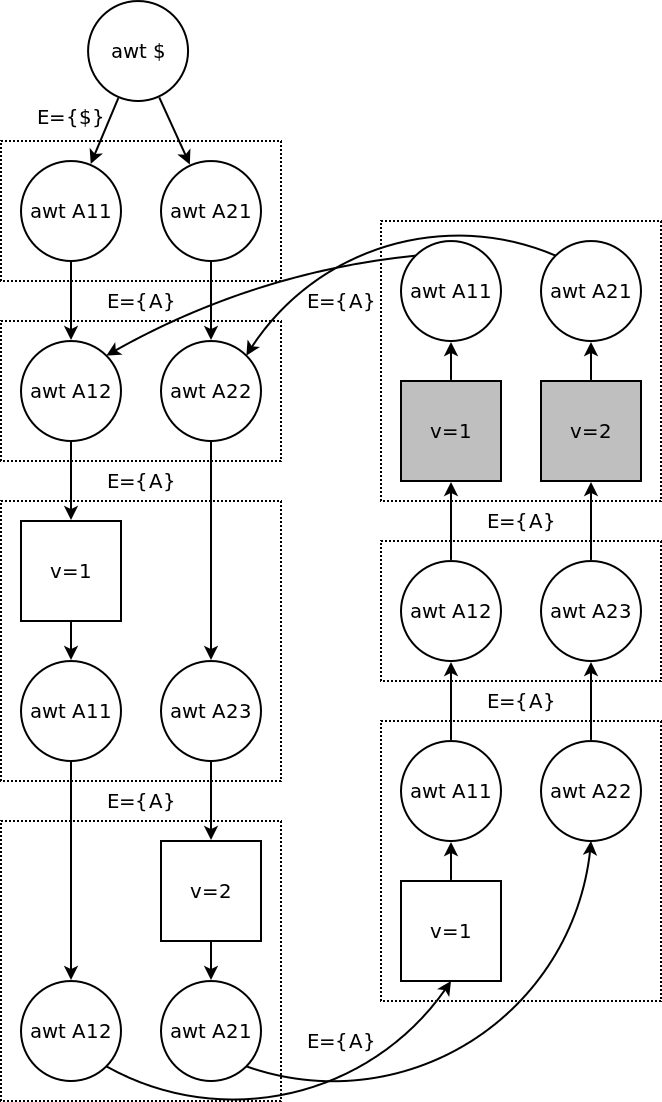
\includegraphics[width=\textwidth]{dfa.png}
\end{minipage}
\caption{ A nondeterministic program in \CEU and its reaction graphs.
\label{fig:det}
}
\end{figure}

Unfortunately, the described algorithm is exponential on the number of 
conditionals and awaits in a program.
Even so, it is applicable for many reasons:

\begin{itemize}
\item Embedded programs are usually small, not being affected by the 
exponential growth.
\item Many programs are safety-critical and must provide as much warranties as 
    possible.
\item The algorithm is easily parallelizable, given that reaction chains do not 
    depend on each other.
\item The development phase \emph{per se} does not require safety warranties, 
reducing considerably the number of times the algorithm has to be executed.
\end{itemize}

Our experience shows that the analysis is indeed practical.
We have been using \CEU in the context of Wireless Sensor 
Networks~\cite{wsn.survey} and applications with around 500 lines of code 
(generating images around 20 Kbytes of ROM) are verified in less than 5 minutes 
(in a \emph{core-duo 2.2~GHz} laptop).

An orthogonal problem to building reaction graphs is to classify $mem$ 
operations that can be safely executed in parallel paths, avoiding false 
positives in the analysis.
For instance, $mem$ operations that accesses different variables can obviously 
execute concurrently.
However, remember from Section~\ref{sec.sem.syntax} that the $mem$ primitive 
represents not only read \& write access to variables, but also $C$ function 
calls.
Moreover, \CEU also supports pointers, which are required for low-level 
manipulation (e.g., accessing buffers from device drivers).

\CEU enforces a default policy for $mem$ operations as follows:
If a variable is written in a path, then a parallel path in the reaction graph 
cannot read or write to that variable, nor dereference a pointer of that 
variable type.
An analogous policy is applied for pointers vs variables and pointers vs 
pointers.
Regarding $C$ calls, they cannot appear in parallel paths, as \CEU has no 
knowledge about their side effects.
Also, passing variables as parameters counts as read accesses to them, while 
passing pointers counts as write accesses to those types (because functions may 
dereference and assign to them).

This policy may still yield some false positives in the analysis.
For instance, the rule for $C$ calls is particularly restrictive, as many 
functions can be safely called concurrently.
Therefore, \CEU supports syntactic annotations that the programmer can use to 
relax the policy explicitly:

\begin{itemize}
\item The \code{pure} modifier declares a $C$ function that does not cause side 
      effects, allowing it to be called concurrently with any other function in 
the program.
\item The \code{det} modifier (for \emph{deterministic}) declares a pair of 
      variables (e.g., pointers) or functions that do not affect each other, 
allowing them to be used concurrently.
\end{itemize}

The following code illustrates \CEU annotations:

{\small
\begin{verbatim}
  pure  _abs;             // 'abs' is side-effect free
  det   _led1 with _led2; // 'led1' vs 'led2' is ok
  int*  buf1, buf2;       // point to different memory
  det   buf1 with buf2;   // 'buf1' vs 'buf2' is ok
\end{verbatim}
}

% TODO: causal, execute/executions

To summarize this section, \CEU only accepts programs with \emph{deterministic 
behavior}, i.e., programs in which any two $mem$ operations identified as 
incompatible (by the prevailing policy) execute only as a causal relation 
between each other in all possible executions.
Therefore, deterministic behavior, as we define, does not require deterministic 
scheduling and can be statically inferred with the presented algorithm.

\subsection{Bounded memory}
\label{sec.safety.mem}

\CEU favors a fine-grained use of trails, being common to use trails that await 
a single event and terminate.
For this reason, \CEU does not allocate per-trail stacks; instead, all locals 
reside in fixed memory slots held in a static one-dimension vector.
Locals for trails in parallel must coexist in memory, while statements in 
sequence can share space.

The memory in \CEU can be precisely calculated, given that programs are defined 
as hierarchies of control-flow statements with explicit forks and joins for 
trails.
This contrasts with threads, which are defined detached from the program 
hierarchy (e.g., a function defined in separate) and requires manual 
bookkeeping (e.g. creation, synchronization, etc.), hindering automatic memory 
prediction and management.

Another concern regarding memory consumption is the runtime stack for internal 
events.
However, note that during runtime, a trail can only occupy one position in the 
stack, given that an emit pauses the trail until the stack unwinds.
Hence, in the worst case, the runtime stack size is the maximum number of 
trails in parallel containing an \code{emit} statement, which is also trivially 
calculated from the program text.

Besides $C$ calls, which are not under control of \CEU, the other possible 
point of failure regarding memory consumption is the queue for external events.
High-frequency external events may fill up the queue before the program can 
react to them, even with the guaranteed bounded execution.
In order to support projects that must deal with event bursts, \CEU delegates 
the queue management to the underlying system, which can provide its own policy 
for adjusting the queue size, prioritizing events, or signaling the program 
about overflows (e.g., through a custom event).

\newpage
\section{Advanced control mechanisms}
\label{sec.adv}

In this section, we explore the stacked execution for internal events in \CEU, 
demonstrating how it enables advanced control-flow mechanisms in the language 
without requiring new primitives.
We first describe a restricted form of subroutines that is used as the basis 
for the more elaborate mechanisms.

Although the described mechanisms involve thoughtful techniques, they can be 
easily abstracted with compile-time macros taking advantage of the structured 
style of \CEU%
\footnote{Our programs in \CEU make extensive use of the \emph{m4} 
preprocessor.}.
As an exception, the \DOFIN construct to be presented in 
Section~\ref{sec.adv.fin} makes slight global additions to the program tree and 
requires a dedicated syntax.

\subsection{Subroutines}
\label{sec.adv.sub}

Internal events bring support for a limited form of subroutines.
In the example that follows, we define a function \code{inc} that increments 
the value passed as reference.
A trail in parallel calls this function in reaction to external event \code{A}:
 
{\small
\begin{verbatim}
 1:  event int* inc;    // function `inc' receives an int
 2:  par/or do
 3:      loop do        // function definitions are loops
 4:          int* p = await inc; // that await the event
 5:          *p = *p + 1;        // to execute the body
 6:      end                     // and await again
 7:  with
 8:      int v = 1;
 9:      await A;
10:      emit inc(&v);           // call `inc'
11:      _assert(v==2);          // assert after return
12:  end
\end{verbatim}
}

A subroutine is represented as a loop that awaits an identifying event 
(\code{await inc}, in line 4).
A subroutine is called in a parallel trail through an emit on the corresponding 
event (\code{emit inc}, in line 10).
The parameter of a subroutine is the type of its corresponding event 
(\code{event int* inc}, in line 1).

In the example, the trails start awaiting events \code{inc} and \code{A}.
Once the input event \code{A} occurs, the second trail awakes and invokes 
\code{emit~inc(\&v)} to ``call'' subroutine \code{f}.
Given the stacked execution for internal events, the calling trail pauses and 
the subroutine awakes.
The subroutine increments the parameter, loops, and awaits to be called again.
Finally, the calling trail resumes and passes the assertion test, terminating 
the program.

This form of subroutines has some significant limitations:

\begin{description}
\item[\emph{Single calling}:] Further calls to a subroutine in a reaction chain 
have no effect.
Suppose that after the assertion test in line 11, the trail tries to call the 
function again.
Given that awaking $await$ statements require them to be $awaiting$ before a 
reaction chain starts, the second call is ignored.
Remember that events are not buffered in \CEU.

\item[\emph{No recursion}:] Recursive calls to a subroutine also have no 
effect.
Suppose that after the increment in line 5, the subroutine tries to call 
itself.
As the trail cannot be awaiting itself while running, the recursive call is 
ignored.

\item[\emph{Single instance}:] Calls to a running subroutine also have no 
effect.
Suppose that after the increment in line 5, the subroutine awaits an event 
(e.g. an external event \code{B}).
While this event does not occur, the subroutine is hanged and cannot serve 
other requests (even in other reaction chains).

\item[\emph{No concurrency}:] If two trails in parallel try to call the same 
subroutine passing a parameter, the static analysis complains about 
nondeterminism.
Considering the formal semantics, an $emit$ needs to be translated to 
$mem;emit(e)$ in order to describe parameter passing (where $mem$ accesses 
$e$).
This way, the concurrent $mem$ operations would be detected as 
nondeterministic.
\end{description}

\vspace{5pt}
\CEU provides no support for standard functions for a number of reasons:
\begin{itemize}
\item The interaction with other \CEU control primitives is not obvious (e.g., 
executing an $await$ or a $par/or$ inside a function).
\item They would still be restricted in some ways given the embedded context 
(e.g.  no recursion or closures).
\item Programs can always recur to $C$ when absolutely necessary.
%\item A dedicated primitive would behave just as described, being a matter of 
%syntactic sugar.
\end{itemize}

Regardless of the limitations, this form of subroutines is widely adopted in 
\CEU programs, given that they were designed to work with the other control 
mechanisms.
Keep in mind that the typical reactive organization of programs (awaiting an 
external stimulus, reacting to it, and going back to awaiting) does not demand 
unrestricted subroutines.
In Section~\ref{sec.adv.frp}, we show that we can even take advantage of 
non-recursive subroutines to properly describe mutual dependency among trails 
in parallel.

\subsection{Finalization blocks}
\label{sec.adv.fin}

Finalization blocks (as found in $Java$ and $C\#$) are often useful to handle 
dynamic resource allocation in a structured way.
As an example, the naive program in \CEU that follows allocates a block of 
memory and uses it across reactions to events before freeing it:

{\small
\begin{verbatim}
    input void A,F;
    par/or do
        tp* ptr = _malloc(...);
        ... // use `ptr'
        await A;
        ... // use `ptr'
        _free(ptr);
    with
        await F;
    end
    ...     // program continues
\end{verbatim}
}

In the program, if event \code{F} occurs before \code{A}, the \code{par/or} 
composition terminates and does not free the allocated memory, leading to a 
leak.

\CEU provides a \DOFIN construct to ensure the execution of a block of code to 
safely release resources.
The previous example can be rewritten as the code in the left side of
Figure~\ref{lst:finally}, which forces the execution of the finalization block 
after the \FIN keyword, even when the outer \code{par/or} terminates.

\DOFIN constructs do not add any complexity to the semantics of \CEU, relying 
only on the set of primitives already presented in 
Section~\ref{sec.sem.syntax}.
% TODO: RW
For instance, the example is translated at compile time into the code shown in 
the right side of the figure, as follows:

\begin{enumerate}
\item A unique global internal event \code{fin} is declared.%
\footnote{Each \DOFIN is associated to an unique event (e.g.,  \code{fin\_1}, 
\code{fin\_2}, etc.).}
\item The \DOFIN is converted into a \code{par/and}.
\item The first \code{par/and} trail emits \code{fin} on termination to invoke 
the finalization block.
\item The second \code{par/and} trail (the finalization block) awaits 
\code{fin} to start executing.
\item All trails that terminate a \code{par/or} or escape a \code{loop} emit 
\code{fin} to also invoke the finalization block.
\end{enumerate}

We opted for a dedicated syntax given that the transformation is not 
self-contained, affecting the global structure of programs.

The cases that follow illustrate the precise behavior of finalization blocks 
when a third trail in parallel encloses a \DOFIN construct and kills it:

\begin{itemize}
\item \emph{3rd trail terminates before the \DOFIN starts to execute.}
In this case, 3rd trail emits the corresponding \code{fin}, which is not yet 
being awaited for, and the finalization block does not execute.
\item \emph{3rd trail terminates while the \DOFIN is blocked.}
In this case, the resource has been acquired but not released.
The corresponding \code{fin} is emitted and holds 3rd trail to awake the 
finalization block, which safely releases the resource before resuming the 
terminating trail.
\item \emph{3rd trail terminates concurrently with the \DOFIN.} (Suppose they 
react to the same event.)
In this case, both trails emit \code{fin}, executing the finalization block 
only once, as expected.
\end{itemize}

\begin{figure}[t]
%\rule{8.5cm}{0.37pt}
{\small
\begin{minipage}[t]{0.45\linewidth}
\begin{alltt}
  input void A,F;

  par/or do
    \textbf{do}
      \_t* ptr = \_malloc();
      ... // use `ptr'
      await A;
      ... // use `ptr'

    \textbf{finally}

      \_free(ptr);
    \textbf{end}
  with
    await F;

  end
\end{alltt}
\end{minipage}
%
\hspace{0.5cm}
%
\begin{minipage}[t]{0.45\linewidth}
\begin{alltt}
input void A,F;
\textbf{event void fin;}      (1)
par/or do
  \textbf{par/and do}          (2)
    \_t* ptr = \_malloc();
    ... // use `ptr'
    await A;
    ... // use `ptr'
    \textbf{emit fin;}        (3)
  \textbf{with}
    \textbf{await fin};       (4)
    \_free(ptr);
  \textbf{end}
with
  await F;
  \textbf{emit fin;}          (5)
end
\end{alltt}
\end{minipage}

\caption{ \DOFIN code and corresponding translation.
\label{lst:finally}
}
}
\end{figure}

%\TODO: limitation: `do´ must await

\DOFIN constructs have the restriction that finalization code cannot await 
events, otherwise they would be killed by the terminating trail before 
releasing the acquired resources.
However, releasing resources does not typically involve awaiting.

\subsection{Exception handling}
\label{sec.adv.excpt}

Exception handling can be provided by specialized programming language 
constructs (e.g., \code{try-catch} blocks in Java), but also with techniques 
using standard control-flow primitives (e.g., \code{setjmp/longjmp} in $C$).
\CEU can naturally express different forms of exception handling without a 
specific construct.

As an illustrative example, suppose an external entity periodically writes to a 
log file and notifies the program through the event \code{ENTRY}, which carries 
the number of available characters to read.
We start with the simple and straightforward specification of 
Figure~\ref{lst:excpt1}.
The normal flow is to open the file and wait in a loop for \code{ENTRY} 
occurrences.
We use a finalization block to safely close the file in the case of abrupt 
terminations, as discussed in previous section.
The low-level file operations \code{open} and \code{read} are defined as 
internal events working as subroutines.
%A \code{read} operation does not await external events, hence, the program 
%loops and awaits event \code{ENTRY} continuously, reacting to all log writes.

\begin{figure}[t]
%\rule{8.5cm}{0.37pt}
{\small
\begin{verbatim}
 // DECLARATIONS
 input int START;  // start handling the log
 input int ENTRY;  // new log entry
 _FILE*    f;      // holds a reference to the log
 char[10] buf;     // holds the current log entry
 event char* open; // opens filename into `f'
 event int read;   // reads a number of bytes into `buf'
 event int excpt;  // callback event for exceptions

 // NORMAL FLOW
 await START;
 do
    emit open("log.txt");
    loop do
       int n = await ENTRY;
       emit read(n);              // reads into `buf'
       _printf("log: %s\n", buf); // handles log string
    end
 finally
    if f != _NULL then
       _fclose(f);
    end
 end
\end{verbatim}
}%
\caption{ Program to handle log entries.
\label{lst:excpt1}
}
\end{figure}

The operations that perform the actual low-level system calls are placed in 
parallel and may emit exceptions through event \code{excpt}, as 
Figure~\ref{lst:excpt2} shows.

\begin{figure}[t]
{\small
\begin{verbatim}
 // DECLARATIONS (as in previous code)
 par/or do
     // NORMAL FLOW (as in previous code)
 with
     loop do     // OPEN subroutine
         char* filename = await open;
         f = _open(filename);
         if f == _NULL then
             emit excpt(1);  // 1 = open exception
         end
     end
 with
     loop do     // READ subroutine
         int n = await read;
         if (n > 10) || (_read(f,buf,n) != n) then
             emit excpt(2);  // 2 = read exception
         end
     end
 end
\end{verbatim}
}%
\caption{ Low-level operations are placed in parallel.
\label{lst:excpt2}
}
\end{figure}

To handle exceptions, we enclose the normal flow with another \code{par/or} to 
terminate it on any exception thrown by file operations:

{\small
\begin{verbatim}
 // DECLARATIONS
 par/or do
     par/or do
         // NORMAL FLOW
     with
         await excpt;    // catch exceptions
     end
 with
     // OPERATIONS       // throw exceptions
 end
\end{verbatim}
}

To illustrate an exception, suppose the normal flow tries to read a string and 
fails.
The program behaves as follows (with the stack in emphasis):

{\small
\begin{enumerate}
\setlength{\itemsep}{0pt}
\item Normal flow invokes the read operation (\code{emit read}) and pauses;\\
    \emph{stack: [norm]}
\item Read operation awakes, throws an exception (\code{emit excpt}), and 
    pauses;\\
    \emph{stack: [norm, read]}
\item Exception handler (\code{await excpt}) awakes, invokes the \FIN (through 
    implicit \code{emit fin}), and pauses;\\
    \emph{stack: [norm, read, hdlr]}
\item The \FIN block executes, closes the file, and terminates;\\
    \emph{stack: [norm, read, hdlr]}
\item The exception continuation terminates the \code{par/or}, cancelling all 
remaining stacked continuations.\\
    \emph{stack: []}
\end{enumerate}
}

This mechanism for exceptions can also support resumption if the handler does 
not terminate its surrounding \code{par/or}.
For instance, the new handler of Figure~\ref{lst:excpt3} waits for exceptions 
in a loop and recovers from each type of exception.

\begin{figure}[t]
{\small
\begin{verbatim}
 ...
     par/or do
         // NORMAL FLOW
     with
         loop do
             int err = await excpt;  // catch exceptions
             if err == 1 then        // open exception
                 f = <creates a new file>
             else/if err == 2 then   // read exception
                 buf = <assigns a default string>
             end
         end
     end
 ...
\end{verbatim}
}%
\caption{ Exception handling with resumption.
\label{lst:excpt3}
}
\end{figure}

Now, step 3 in the previous execution trace would not fire the \FIN block, but 
instead, assign a default string to \code{buf}, loop and await the next 
exception.
Then, the exception continuation would loop and await further file operations.
In the end, the read operation would resume as if no exceptions had occurred.

Note that throughout the example, the normal flow of Figure~\ref{lst:excpt1} 
remained unchanged, with all machinery to handle exceptions placed around it.
Also, although we use globals in the example (\code{f} and \code{buf}), 
remember that they are guaranteed to be safely accessed.
%The only modification was actually a bug removal, as we included the 
%\code{do-finally} block to ensure closing the file safely.

In terms of memory usage, switching from the original normal flow (without 
exception throws) to the last example (with recovery) incurred extra 450 bytes 
of ROM and 24 bytes of RAM.

The presented approach for exceptions has the limitation that a file operation 
cannot be called twice within a reaction chain and that exception handlers 
cannot await other events, which are related to the single-call and 
single-instance property of subroutines in \CEU.

\subsection{Dataflow programming}
\label{sec.adv.frp}

Reactive dataflow programming \cite{frp.survey} provides a declarative style to 
express dependency relationships among data.
Mutual dependency is a known issue in dataflow languages, requiring the 
explicit placement of a specific delay operator to avoid runtime
cycles~\cite{frtime.embedding,luagravity.sblp}.
This solution is somewhat \emph{ad hoc} and splits an internal dependency 
problem across two reactions to the environment.
%It also requires the mutual dependency to eventually converge to a value so 
%that variables do not affect each other forever.

\CEU can naturally express safe mutual dependencies, making it impossible to 
implement recursive definitions (as shown in Section~\ref{sec.safety.bounded}).
For instance, the program in Figure~\ref{lst:ceu:frp:2} applies the temperature 
conversion formula between Celsius and Fahrenheit, so that whenever the value 
in one unit is set, the other is automatically recalculated (a problem proposed 
in~\cite{frp.survey}).

\begin{figure}[t]
%\rule{8.5cm}{0.37pt}
{\small
\begin{verbatim}
 1:   event int TC, TF;
 2:   int tc, tf;
 3:   event int tc_evt, tf_evt;
 4:   par/or do
 5:      loop do                // 1st trail
 6:         tc = await tc_evt;
 7:         emit tf_evt(9 * tc / 5 + 32);
 8:      end
 9:   with
10:      loop do                // 2nd trail
11:         tf = await tf_evt;
12:         emit tc_evt(5 * (tf-32) / 9);
13:      end
14:   with
15:      loop do
16:         int v = await TC;   // 3rd trail
17:         emit tc_evt(v);
18:         ...   // use `tc' or `tf'
19:      end
20:   with
21:      loop do
22:         int v = await TF;   // 4th trail
23:         emit tf_evt(v);
24:         ...   // use `tc' or `tf'
25:      end
26:   end
\end{verbatim}
}%
\caption{ A dataflow program with mutual dependency.
\label{lst:ceu:frp:2}
}
\end{figure}

We first define the external events that signal changes, the variables to hold 
the temperatures, and corresponding internal events (lines 1-3).
Any change to a variable in the program must be signalled by an emit on the 
corresponding internal event so that dependent variables can react.
Then, we create two trails to await for internal changes and update the 
dependency relations among the temperatures (lines 5-8 and 10-13).
For instance, the first trail is a \code{loop} that waits for changes on 
\code{tc\_evt} (line 6) and signals the conversion formula to \code{tf\_evt} 
(line 7).
The behavior for the second trail that awaits \code{tf\_evt} (lines 10-13) is 
analogous.
The third and fourth trails (lines 15-19 and 21-25) await external updates in
loop to notify the internal changes;
The program behaves as follows (with the stack in emphasis):

{\small
\begin{enumerate}
\setlength{\itemsep}{0pt}
\item 1st and 2nd trail await \code{tc\_evt} and \code{tf\_evt};\\
    \emph{stack: []}
\item If \code{TC} occurs, 3rd trail signals a change to \code{tc\_evt} and 
    pauses;\\
    \emph{stack: [3rd]}
\item 1st trail awakes, sets \code{tc=0}, emits \code{tf\_evt}, and pauses;\\
    \emph{stack: [3rd,1st]}
\item 2nd trail awakes, sets \code{tf=32}, emits \code{tc\_evt}, and pauses;\\
    \emph{stack: [3rd,1st,2nd]}
\item no trails are awaiting \code{tc\_evt} (1st trail is paused), so 2nd trail 
    (on top of the stack) resumes, loops, and awaits \code{tf\_evt} again;\\
    \emph{stack: [3rd,1st]}
\item 1st trail resumes, loops, and awaits \code{tc\_evt} again;\\
    \emph{stack: [3rd]}
\item 3rd trail resumes \emph{with all dependencies resolved} and awaits the 
    next external change;\\
    \emph{stack: []}
\item ... (analogous behavior for further external occurrences)
\end{enumerate}
}

The complexity of the solution is disproportionate to the problem it solves, 
but illustrates the circular dependency issue (similar examples appear in other 
references~\cite{frp.survey,frtime.embedding}).
The bottom line is that dataflow techniques permit that complex dependency 
patterns are handled internally, providing well-defined entry points to 
application programmers (i.e. they would be required to write only the 3rd and 
4th trails in the example).

%Altough xxx, no support for dynamic reconfiguration given the static nature of

%\newpage
%\section{Implementation of \CEU}

%\newpage
\section{Related work}
\label{sec.related}

\CEU is strongly influenced by Esterel~\cite{esterel.ieee91}, but they are 
different in the fundamental aspect of dealing with events (signals in 
Esterel).
For instance, the stacked execution for internal events employed by \CEU 
greatly improves the expressiveness of the language as shown in 
Section~\ref{sec.adv}.
%For instance, dataflow programming is not feasible in Esterel, what resulted 
%in dedicated languages for that purpose~\cite{rp.twelve}.

Furthermore, Esterel is commonly used in hardware design, and its notion of 
time is similar to that of digital circuits, where multiple signals can be 
active at a clock tick.
In \CEU, instead of clock ticks, the occurrences of external events that define 
time units.
We believe that for software design, this approach simplifies the reasoning 
about concurrency.
For instance, the uniqueness of external events in \CEU is a prerequisite for 
its static analysis that enables safe shared-memory concurrency.
However, in Esterel, \emph{if a variable is written by some thread, then it can 
neither be read nor be written by concurrent threads}~\cite{esterel.primer} 
(this statement regards to the program text, not to a reaction chain).

More recently, Wireless Sensor Networks (WSNs) emerged as an active research 
area for highly constrained embedded concurrency, resulting in the development 
of many synchronous languages~\cite{wsn.protothreads,wsn.sol,wsn.osm}.

Protothreads \cite{wsn.protothreads} offer lightweight cooperative 
multithreading for embedded systems.
Its stackless implementation reduces memory consumption but precludes support 
for local variables.
\CEU also avoids the use of stacks for trails, but preserves support for locals 
by calculating the required memory at compile time.
%, as shown in Section~\ref{sec.safety.mem}.

SOL~\cite{wsn.sol} and OSM~\cite{wsn.osm} provide parallel state machines for 
WSNs, offering a formal and mature model for programming embedded systems.
However, the main contributions of \CEU, stacked execution for internal 
events and safe support for shared-memory concurrency, do not directly adapt to 
the state-machine formalism.

In common among the referred works is the agreement in providing low-level 
access (e.g., systems calls and shared-memory) and lock-free concurrency that 
precludes race conditions on programs.
However, they do not specify an execution order for tasks reacting to the same 
external stimulus~\cite{esterel.primer,wsn.protothreads,wsn.osm}.
This way, if two tasks access the same resource concurrently, even if the 
accesses are race free, the final outcome is nondeterministic.
As discussed in Section~\ref{sec.safety.det}, \CEU refuses programs with such 
behavior.

%{\small
%\begin{itemize}
%\item \emph{If there is no control dependency and no signal dependency, as in 
%\code{(call~P1()~||~call~P2())}, the order is unspecified and it would be an
%error to rely on it.}~\cite{esterel.primer}
%\item \emph{The protothreads mechanism does not specify any specific method to 
%invoke or schedule a protothread, this is defined by the system using 
%protothreads.}~\cite{wsn.protothreads}
%\item \emph{A single write access will always completely execute before the 
%next write access can occur. However, the order in which write accesses are 
%executed is arbitrary.}~\cite{wsn.osm}
%\item \emph{The parallel operator executes all its threads in a round-robin 
%manner according to the order of their declaration in the 
%program.}~\cite{wsn.sol}
%\end{itemize}
%}

%Regarding the last policy, we believe that our proposed static analysis is an 
%improvement over deterministic schedulers.

On the opposite side of the spectrum of concurrency models, asynchronous 
languages for embedded systems~\cite{wsn.mantisos,arduino.occam}
assume time independence among processes and are more appropriate for 
applications with a low synchronization rate or for those involving
algorithmic-intensive problems.

\begin{comment}
% TODO
SHIM is an asynchronous language that enforces synchronous communications among 
processes, providing a deterministic execution model.
SHIM distinguishes from typical asynchronous languages given that
The use of point-to-point communication, typical in CSP-like 
languages~\cite{async.csp}, leads to a different programming mindset.
No shared-memory
no hierarchies (e.g., \code{par/or} compositions)
\end{comment}

%TODO: limitation static (mantis, proto, occam tb!)

% TODO: leds, buffer overflows

Asynchronous models are also employed in real-time operating systems to provide 
response predictability, typically through prioritized 
schedulers~\cite{wsn.mantisos,wsn.oses,freertos}.
Even though \CEU ensures bounded execution for reactions, it cannot provide 
hard real-time warranties.
For instance, assigning different priorities for trails would break lock-free 
concurrency (i.e., breaking correctness is worse than breaking timeliness).
%synchronous model and
%the static analysis, which are required for

%That said, some embedded systems do require prioritized scheduling to meet 
%deadlines for critical tasks, even if it involves extra complexity to deal 
%%with synchronization issues.
Fortunately, \CEU and RTOSes are not mutually exclusive, and we can foresee a 
scenario in which multiple \CEU programs run in different RTOS threads and 
communicate asynchronously via external events, an architecture known as GALS 
(\emph{globally asynchronous--locally synchronous})~\cite{rp.gals}.

Concerning the described control-flow mechanisms, they heavily rely on 
\code{par/or} compositions, which cannot be precisely defined in asynchronous 
languages without tweaking processes with synchronization 
mechanisms~\cite{esterel.preemption}.

Finally, although \CEU provides some dataflow functionality, it is not intended 
for data-intensive applications.
For instance, the \emph{Functional Reactive Programming (FRP)} is a more 
expressive paradigm with this respect, supporting the dynamic creation of 
signals at runtime~\cite{frp.principles}.
We believe that dataflow and imperative reactivity are complementary, but the 
latter is more suitable for control-intensive embedded systems that must deal 
with low-level I/O and handle explicit state.

\section{Conclusion}
\label{sec.conclusion}

In this work, we presented a formal description of the control aspects of the 
reactive programming language \CEU and discussed how to detect unsafe 
properties of programs at compile time.
\CEU is based on Esterel, but introduces the stacked behavior for internal 
events and the static analysis for shared-memory concurrency.

\CEU achieves a high degree of reliability for embedded systems, while also 
embraces practical aspects, such as support for lock-free concurrency, 
low-level access to the platform, and advanced control-flow mechanisms.

We consider that providing safe shared-memory concurrency is a fundamental 
design choice of \CEU, given that low-level I/O is indispensable in the context 
of embedded systems (e.g. interfacing with sensors and actuators).

Embedded systems are still predominantly developed in the ``bare metal'', 
regardless of existing alternatives, probably due to the flexibility and 
popularity of $C$.
We believe that \CEU is an attractive alternative, given its unrestricted 
access to $C$ and rich set of concurrent control primitives (e.g., parallel 
compositions and internal events).

\begin{comment}
Currently, \CEU is not intended for use in other reactive scenarios, such as 
desktop applications and games:
besides the impracticability of the static analysis for larger applications, 
\CEU does not support the dynamic creation of trails, which is essential for 
virtualizing resources (e.g., graphical widgets, AI units, etc.).

most bug are in control aspects
spaghetti code
not on C calls

static
no virtualization of devices
1x1

Main contribution, stacked execution,
fundamental for the bounded execution (used on proof)
and for deriving control primitives

TODO: evaluation
- compared to handcrafted...

- Non-features
    - exponential analysis

the static analysis also detects the exact mem size
it is impossible to overflow timers/spawns
looks like dynamic but it is not
optionally, defensive (just count the number)

\CEU still has the limitation of not creating new lines of execution at runtime
They are all known in advance to properly calculate the amount of memory
also, dynamic would require a more complex static analysis
Note that dynamically allocating threads is not common in ES (chibi, what 
else?)

On the way to a more in-depth qualitative approach, we are currently teaching 
\CEU{} as an alternative to \nesc{} in a hands-on WSN course in a high-school.
The students successfully implemented a simple multi-hop communication protocol 
in \CEU.
Also, the same format is being employed in an undergraduate course, but still 
in an early stage.
We will compare the achievements of the students with both languages and use 
the results in our evaluation.

\end{comment}

%\newpage
\bibliographystyle{abbrvnat}
%\small{
\bibliography{other,my}
%}

\begin{comment}
The examples in Figure~\ref{lst:subs} show how this form of subroutines has 
some significant limitations.
We assume that the bodies represented as \code{...} do not contain \code{await} 
statements (but example~\ref{lst:subs}.c explicitly includes one).
Once again, the external event \code{A} represents the reaction that ``calls'' 
the functions.

The example~\ref{lst:subs}.a shows that a subroutine can be called only a 
single time during a reaction chain (further calls have no effect):
The first trail calls \code{f} in reaction to \code{A} and blocks.
After the subroutine returns, the first trail tries to call the function again.
However, given that $await$ statements must be previously awaiting to react to 
an $emit$, the second call is ignored.

The example~\ref{lst:subs}.b shows that subroutines are non-recursive 
(recursive calls have no effect):
The recursive call in the first trail fails, because the subroutine is not 
awaiting event \code{g} in the moment its body calls itself.
Remember that events are unbuffered in \CEU.
The recursive call fails, but the subsequent call in reaction to the next 
occurrence of \code{A} behaves normally.

The example~\ref{lst:subs}.c shows that subroutines can only run a single 
instance at a time (calls to running subroutines have no effect):
The first trail calls \code{h}, which awaits event \code{i} in its body.
The second reaction to \code{A} calls the subroutine again.
However, the subroutine did not terminate and the second call is missed.

\begin{figure}[t]
%\rule{8.5cm}{0.37pt}
{\small
\begin{minipage}[t]{0.25\linewidth}
\begin{verbatim}
 input void A;
 event void f;
 par/or do
   loop do
     await f;
     ...
   end

 with
   await A;
   emit f;
   emit f;
 end


     (6.a)
  single call
\end{verbatim}
\end{minipage}
%
\hspace{0.7cm}
%
\begin{minipage}[t]{0.25\linewidth}
\begin{verbatim}
input void A;
event void g;
par/or do
  loop do
    await g;
    ...
    emit g;
  end
with
  await A;
  emit g;
  await A;
  emit g;
end

    (6.b)
non-recursive
\end{verbatim}
\end{minipage}
\hspace{0.7cm}
%
\begin{minipage}[t]{0.25\linewidth}
\begin{verbatim}
input void A;
event void h,i;
par/or do
  loop do
    await h;
    ...
    await i;
  end
with
  await A;
  emit h;
  await A;
  emit h;
end

    (6.c)
single instance
\end{verbatim}
\end{minipage}
\caption{ Subroutines in \CEU.
\label{lst:subs}
}
}
\end{figure}
\end{comment}

\end{document}
